\documentclass{beamer}
\usetheme{Madrid}
\usecolortheme{beaver}
\usepackage{tikz}
\usepackage{amsmath}
\usepackage{amssymb}
\usepackage{bussproofs}
\usepackage{array}

\title{Basic Proofs in Predicate Logic}
\subtitle{Building Arguments Step by Step}
\author{Brendan Shea, PhD}
\date{Intro to Logic}

\begin{document}
	
	% Slide 1: Title Slide
	\begin{frame}
		\titlepage
	\end{frame}
	
	% Slide 2: What Is a Proof?
	\begin{frame}{What Is a Proof? Building Logical Bridges}
		\begin{itemize}
			\item A \textbf{proof} is a sequence of logical steps showing a conclusion \textbf{must} be true given certain premises.
			\item Proofs are \textbf{deductive}: they preserve truth with 100\% certainty from premises to conclusion.
			\item Each step follows by a \textbf{rule of inference}—a logical principle that guarantees truth preservation.
			\item Unlike inductive reasoning (probable conclusions) or abductive reasoning (best explanations), deductive proofs offer absolute certainty!
		\end{itemize}
		
		\begin{block}{Deductive Certainty}
			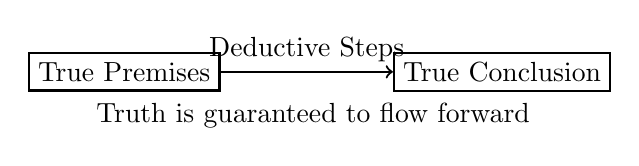
\begin{tikzpicture}[scale=0.8]
				\node[rectangle,draw,thick] (start) at (0,0) {True Premises};
				\node[rectangle,draw,thick] (end) at (6,0) {True Conclusion};
				\draw[->,thick] (start) -- (end) node[midway,above] {Deductive Steps};
				\node at (3,-0.7) {Truth is guaranteed to flow forward};
			\end{tikzpicture}
		\end{block}
	\end{frame}
	
	% Slide 3: Why Proofs Matter
	\begin{frame}{Why Proofs Matter: From Ancient Geometry to Modern Cryptography}
		\begin{itemize}
			\item \textbf{Mathematics}: Proofs ensure that mathematical facts are eternally true, not just probably true.
			\item \textbf{Computer Security}: Your online banking is safe because of mathematical proofs about encryption.
			\item \textbf{Science}: Proofs help us distinguish between correlation and causation in research.
			\item \textbf{Critical Thinking}: Learning to prove things makes you immune to logical fallacies and bad arguments.
		\end{itemize}
		
		\begin{example}
			Real-world applications of proofs:
			\begin{itemize}
				\scriptsize
				\item Proving that a sorting algorithm always works correctly
				\item Proving that a medical treatment actually causes improvement
				\item Proving that a voting system is fair and can't be manipulated
				\item Proving that a bridge design can support its maximum load
			\end{itemize}
		\end{example}
	\end{frame}
	
	% Slide 4: Proofs vs Persuasion
	\begin{frame}{Proofs vs. Persuasion: The Gold Standard of Certainty}
		\begin{itemize}
			\item \textbf{Deductive proof}: Guarantees truth—if premises are true, conclusion MUST be true.
			\item \textbf{Inductive reasoning}: Suggests probability—"All swans I've seen are white, so probably all swans are white."
			\item \textbf{Abductive reasoning}: Offers best explanation—"The grass is wet, so it probably rained."
			\item Only deductive proofs provide absolute certainty; the others give us useful but fallible conclusions.
		\end{itemize}
		
		\begin{alertblock}{Types of Reasoning}
			\scriptsize{
			\begin{tabular}{|l|l|l|}
				\hline
				\textbf{Type} & \textbf{Example} & \textbf{Certainty} \\
				\hline
				Deductive & All birds have wings; X is a bird; so X has wings & 100\% \\
				Inductive & I've seen 1000 white swans; next one is probably white & High probability \\
				Abductive & Patient has symptoms A,B,C; likely has disease D & Best guess \\
				\hline
			\end{tabular}
		}
		\end{alertblock}
	\end{frame}
	
	% Slide 5: The Structure of a Formal Proof
	\begin{frame}{The Structure of a Formal Proof: Steps and Justifications}
		\begin{itemize}
			\item Every proof consists of numbered lines, each containing a \textbf{statement} and its \textbf{justification}.
			\item Justifications can be: premises (given), rules of inference, or references to previous lines.
			\item Each line follows logically from previous lines according to specific rules.
			\item The last line of the proof is your conclusion—what you set out to prove!
		\end{itemize}
		
		\begin{block}{Anatomy of a Proof}
			\begin{tabular}{|c|l|l|}
				\hline
				\textbf{Line} & \textbf{Statement} & \textbf{Justification} \\
				\hline
				1 & $P \rightarrow Q$ & Premise \\
				2 & $P$ & Premise \\
				3 & $Q$ & Modus Ponens (1,2) \\
				\hline
			\end{tabular}
			
			This proves: From "If $P$ then $Q$" and "$P$", we can conclude "$Q$"
		\end{block}
	\end{frame}
	
	% Slide 6: Valid Arguments
	\begin{frame}{Valid Arguments: When Conclusions Must Follow}
		\begin{itemize}
			\item An argument is \textbf{valid} if the conclusion must be true whenever all premises are true.
			\item Validity is about the structure of the argument, not whether premises are actually true.
			\item A valid argument with true premises is called \textbf{sound}—this guarantees a true conclusion.
			\item Our proof rules preserve validity: applying them to true statements always yields true statements.
		\end{itemize}
		
		\begin{example}
			Valid argument (even with silly premises):
			\begin{enumerate}
				\item All creatures in Wonderland can talk (premise)
				\item The Cheshire Cat is in Wonderland (premise)
				\item Therefore, the Cheshire Cat can talk (conclusion)
			\end{enumerate}
			The structure is valid: All A's are B, X is an A, therefore X is B.
		\end{example}
	\end{frame}
	
	% Slide 7: Common Proof Mistakes
	\begin{frame}{Common Proof Mistakes: Learning from Logical Missteps}
		\begin{itemize}
			\item \textbf{Circular reasoning}: Using what you're trying to prove as a justification.
			\item \textbf{Unjustified jumps}: Skipping steps that seem "obvious" but need proof.
			\item \textbf{Wrong rule application}: Using a rule incorrectly or in the wrong situation.
			\item \textbf{Assuming the converse}: Thinking "If $P$ then $Q$" means "If $Q$ then $P$".
		\end{itemize}
		
		\begin{alertblock}{Classic Mistakes to Avoid}
			\begin{itemize}
				\item "Everyone knows that..." — Not a valid justification!
				\item Going from "Some cats are black" to "Fluffy is black" — Need more info!
				\item Using $P \rightarrow Q$ backwards — Can't conclude $P$ from $Q$!
				\item Forgetting to cite line numbers — Every step needs justification!
			\end{itemize}
		\end{alertblock}
	\end{frame}
	
	% Slide 8: Your First Proof
	\begin{frame}{Your First Proof: A Simple Example to Get Started}
		\begin{itemize}
			\item Let's prove: "Dorothy has silver shoes and wants to go home, so Dorothy wants to go home."
			\item Premises: (1) Dorothy has silver shoes AND Dorothy wants to go home
			\item Conclusion: Dorothy wants to go home
			\item We'll use our first rule: \textbf{conjunction elimination} (taking AND statements apart).
		\end{itemize}
		
		\begin{example}
			\scriptsize{
			\begin{tabular}{|c|l|l|}
				\hline
				\textbf{Line} & \textbf{Statement} & \textbf{Justification} \\
				\hline
				1 & \texttt{HasSilverShoes(Dorothy)} $\land$ \texttt{WantsHome(Dorothy)} & Premise \\
				2 & \texttt{WantsHome(Dorothy)} & $\land$ Elimination (1) \\
				\hline
			\end{tabular}
			
			We extracted the second part of the AND statement—our first proof is complete!
		}
		\end{example}
	\end{frame}
	
	% Slide 9: The Toolbox
	\begin{frame}{The Toolbox: Introduction and Elimination Rules}
		\begin{itemize}
			\item For each logical operator, we have two types of rules: \textbf{introduction} and \textbf{elimination}.
			\item \textbf{Introduction rules} show how to prove statements with that operator.
			\item \textbf{Elimination rules} show how to use statements with that operator.
			\item Think of it like a toolbox: some tools build things up, others take them apart!
		\end{itemize}
		
		\begin{block}{Rules for Each Operator}
			\begin{tabular}{|c|c|c|}
				\hline
				\textbf{Operator} & \textbf{Introduction} & \textbf{Elimination} \\
				\hline
				$\land$ (and) & Combine statements & Extract parts \\
				$\lor$ (or) & Add possibilities & Consider cases \\
				$\rightarrow$ (if-then) & Assume and derive & Apply condition \\
				$\neg$ (not) & Show contradiction & Cancel double negative \\
				\hline
			\end{tabular}
		\end{block}
	\end{frame}
	
	% Slide 10: Conjunction Introduction
	\begin{frame}{Conjunction Introduction: Building "And" Statements}
		\begin{itemize}
			\item \textbf{Conjunction Introduction} ($\land$I): If you've proved $P$ and you've proved $Q$, you can conclude $P \land Q$.
			\item This rule lets us combine separate facts into a single compound statement.
			\item Symbol: $\frac{P \quad Q}{P \land Q}$ (from $P$ and $Q$ separately, infer $P \land Q$).
			\item The most straightforward rule—if you know both parts, you know the whole!
		\end{itemize}
		
		\begin{example}
			\scriptsize{
			Rule in action:
			\begin{tabular}{|c|l|l|}
				\hline
				\textbf{Line} & \textbf{Statement} & \textbf{Justification} \\
				\hline
				1 & \texttt{InKansas(Dorothy)} & Premise \\
				2 & \texttt{HasDog(Dorothy, Toto)} & Premise \\
				3 & \texttt{InKansas(Dorothy)} $\land$ \texttt{HasDog(Dorothy, Toto)} & $\land$I (1,2) \\
				\hline
			\end{tabular}
		}
		\end{example}
	\end{frame}
	
	
	
	% Slide 11: Proving Dorothy Has Ruby Slippers AND Wants to Go Home
	\begin{frame}{Proving Dorothy Has Ruby Slippers AND Wants to Go Home: Conjunction Introduction Practice}
		\begin{itemize}
			\item Given: (1) Dorothy has ruby slippers, (2) Dorothy wants to go home
			\item Goal: Prove that Dorothy has ruby slippers AND wants to go home
			\item Strategy: Use conjunction introduction to combine the two given facts.
			\item This shows how we build complex statements from simpler ones.
		\end{itemize}
		
		\begin{block}{The Proof}
			\scriptsize{
			\begin{tabular}{|c|l|l|}
				\hline
				\textbf{Line} & \textbf{Statement} & \textbf{Justification} \\
				\hline
				1 & \texttt{HasRubySlippers(Dorothy)} & Premise \\
				2 & \texttt{WantsHome(Dorothy)} & Premise \\
				3 & \texttt{HasRubySlippers(Dorothy)} $\land$ \texttt{WantsHome(Dorothy)} & $\land$I (1,2) \\
				\hline
			\end{tabular}
			
			Notice how line 3 references both lines 1 and 2—we need both pieces!
		}
		\end{block}
	\end{frame}
	
	% Slide 12: Conjunction Elimination
	\begin{frame}{Conjunction Elimination: Taking "And" Statements Apart}
		\begin{itemize}
			\item \textbf{Conjunction Elimination} ($\land$E): From $P \land Q$, you can conclude $P$ or conclude $Q$ (or both).
			\item This rule lets us extract useful information from compound statements.
			\item Two forms: $\frac{P \land Q}{P}$ (left elimination) and $\frac{P \land Q}{Q}$ (right elimination).
			\item Like unpacking a box—if the box contains both items, you can take out either one!
		\end{itemize}
		
		\begin{alertblock}{Using $\land$E}
			\scriptsize{
			From "\texttt{IsWitch(Glinda)} $\land$ \texttt{IsGood(Glinda)}":
			\begin{itemize}
				\item We can conclude \texttt{IsWitch(Glinda)} (left part)
				\item We can conclude \texttt{IsGood(Glinda)} (right part)
				\item We can use both conclusions in our proof!
			\end{itemize}
		}
		\end{alertblock}
	\end{frame}
	% Slide 13: From Complex to Simple
	\begin{frame}{From Complex to Simple: Conjunction Elimination Practice}
		\begin{itemize}
			\item Given: The Scarecrow wants a brain AND is made of straw AND can talk
			\item Goal: Prove that the Scarecrow can talk
			\item Strategy: Use conjunction elimination to extract the part we need.
			\item With nested conjunctions, we may need multiple elimination steps!
		\end{itemize}
		
		\begin{example}
			\begin{tabular}{|c|l|l|}
				\hline
				\textbf{Line} & \textbf{Statement} & \textbf{Justification} \\
				\hline
				1 & (\texttt{WantsBrain(Scarecrow)} $\land$ \texttt{MadeOfStraw(Scarecrow)}) & \\
				& $\land$ \texttt{CanTalk(Scarecrow)} & Premise \\
				2 & \texttt{CanTalk(Scarecrow)} & $\land$E (1) \\
				\hline
			\end{tabular}
			
			We extracted the rightmost part of the complex conjunction!
		\end{example}
	\end{frame}
	
	% Slide 14: Disjunction Introduction
	\begin{frame}{Disjunction Introduction: Creating "Or" Statements}
		\begin{itemize}
			\item \textbf{Disjunction Introduction} ($\lor$I): If you've proved $P$, you can conclude $P \lor Q$ for any $Q$.
			\item This might seem strange—we're adding uncertainty where there was none!
			\item But it's logically valid: if $P$ is true, then "$P$ or $Q$" must be true (regardless of $Q$).
			\item Useful when you need to match a specific form or work with given disjunctions.
		\end{itemize}
		
		\begin{block}{Two Forms of $\lor$I}
			\begin{itemize}
				\item From $P$, conclude $P \lor Q$ (left introduction)
				\item From $Q$, conclude $P \lor Q$ (right introduction)
			\end{itemize}
			Example: From "Alice is in Wonderland", we can conclude "Alice is in Wonderland OR Alice is in Oz"
		\end{block}
	\end{frame}
	
	% Slide 15: Proving The Cat Is Grinning OR Invisible
	\begin{frame}{Proving "The Cat Is Grinning OR Invisible": Disjunction Introduction Practice}
		\begin{itemize}
			\item Given: The Cheshire Cat is grinning
			\item Goal: Prove that the Cheshire Cat is grinning OR the Cheshire Cat is invisible
			\item Strategy: Use disjunction introduction to add the alternative possibility.
			\item Remember: We're not claiming the cat is invisible—just that at least one option is true!
		\end{itemize}
		
		\begin{example}
			\scriptsize{
			\begin{tabular}{|c|l|l|}
				\hline
				\textbf{Line} & \textbf{Statement} & \textbf{Justification} \\
				\hline
				1 & \texttt{IsGrinning(CheshireCat)} & Premise \\
				2 & \texttt{IsGrinning(CheshireCat)} $\lor$ \texttt{IsInvisible(CheshireCat)} & $\lor$I (1) \\
				\hline
			\end{tabular}
			
			Even though we only know the cat is grinning, the "or" statement is certainly true!
		}
		\end{example}
	\end{frame}
	
	% Slide 16: Disjunction Elimination
	\begin{frame}{Disjunction Elimination: The Case-by-Case Method}
		\begin{itemize}
			\item \textbf{Disjunction Elimination} ($\lor$E): The most complex rule so far—reasoning by cases.
			\item If you know $P \lor Q$, and you can prove $R$ from $P$, and prove $R$ from $Q$, then $R$ must be true.
			\item Think: "Either way, we get the same result, so that result must hold."
			\item Requires setting up two sub-proofs, one for each possibility.
		\end{itemize}
		
		\begin{alertblock}{Structure of $\lor$E}
			\small
			To use $P \lor Q$:
			\begin{enumerate}
				\item Assume $P$ temporarily, prove $R$
				\item Assume $Q$ temporarily, prove $R$
				\item Conclude $R$ (since it follows either way)
			\end{enumerate}
			Like checking both paths at a fork in the road and finding they lead to the same place!
		\end{alertblock}
	\end{frame}
	
	% Slide 17: Working Through Cases
	\begin{frame}{Working Through Cases: Disjunction Elimination Practice}
		\begin{itemize}
			\item Given: Either the Tin Man needs oil OR he needs a heart
			\item Given: If he needs oil, he can't move. If he needs a heart, he can't love.
			\item Goal: Prove that either he can't move OR he can't love
			\item Strategy: Consider both cases and show each leads to our conclusion.
		\end{itemize}
		
		\begin{example}
			\footnotesize
			\begin{tabular}{|c|l|l|}
				\hline
				1 & \texttt{NeedsOil(TinMan)} $\lor$ \texttt{NeedsHeart(TinMan)} & Premise \\
				2 & \texttt{NeedsOil(TinMan)} $\rightarrow$ \texttt{CantMove(TinMan)} & Premise \\
				3 & \texttt{NeedsHeart(TinMan)} $\rightarrow$ \texttt{CantLove(TinMan)} & Premise \\
				\hline
				4 & \quad \texttt{NeedsOil(TinMan)} & Assume (for $\lor$E) \\
				5 & \quad \texttt{CantMove(TinMan)} & Modus Ponens (2,4) \\
				6 & \quad \texttt{CantMove(TinMan)} $\lor$ \texttt{CantLove(TinMan)} & $\lor$I (5) \\
				\hline
				7 & \quad \texttt{NeedsHeart(TinMan)} & Assume (for $\lor$E) \\
				8 & \quad \texttt{CantLove(TinMan)} & Modus Ponens (3,7) \\
				9 & \quad \texttt{CantMove(TinMan)} $\lor$ \texttt{CantLove(TinMan)} & $\lor$I (8) \\
				\hline
				10 & \texttt{CantMove(TinMan)} $\lor$ \texttt{CantLove(TinMan)} & $\lor$E (1,4-6,7-9) \\
				\hline
			\end{tabular}
		\end{example}
	\end{frame}
	
	% Slide 18: Conditional Introduction
	\begin{frame}{Conditional Introduction: Building "If-Then" Statements}
		\begin{itemize}
			\item \textbf{Conditional Introduction} ($\rightarrow$I): To prove $P \rightarrow Q$, assume $P$ and derive $Q$.
			\item This captures how we naturally think about "if-then": "If this were true, what would follow?"
			\item The assumption is temporary—only valid within the sub-proof.
			\item Once we derive $Q$ from the assumption $P$, we can conclude $P \rightarrow Q$ outside the sub-proof.
		\end{itemize}
		
		\begin{block}{The Power of Assumption}
			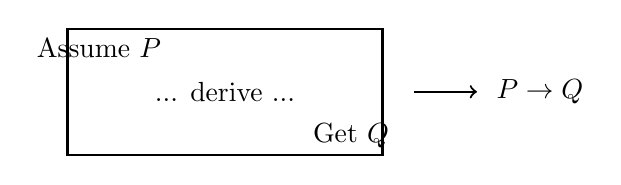
\begin{tikzpicture}[scale=0.8]
				\draw[thick] (0,0) rectangle (5,2);
				\node at (0.5,1.7) {Assume $P$};
				\node at (2.5,1) {... derive ...};
				\node at (4.5,0.3) {Get $Q$};
				\draw[->,thick] (5.5,1) -- (6.5,1);
				\node at (7.5,1) {$P \rightarrow Q$};
			\end{tikzpicture}
		\end{block}
	\end{frame}
	
	% Slide 19: Proving If You Click Your Heels Three Times
	\begin{frame}{Proving "If You Click Your Heels Three Times, Then You'll Go Home": Conditional Introduction}
		\begin{itemize}
			\item Given: Anyone who clicks their heels three times while wearing ruby slippers goes home
			\item Given: Dorothy has ruby slippers
			\item Goal: If Dorothy clicks her heels three times, then Dorothy goes home
			\item Strategy: Assume the "if" part and derive the "then" part.
		\end{itemize}
		
		\begin{example}
			\scriptsize{
			\begin{tabular}{|c|l|l|}
				\hline
				1 & $\forall x$ ((\texttt{ClicksHeels3x}$(x) \land$ \texttt{HasRubySlippers}$(x))$ & \\
				& $\rightarrow$ \texttt{GoesHome}$(x)$) & Premise \\
				2 & \texttt{HasRubySlippers(Dorothy)} & Premise \\
				\hline
				3 & \quad \texttt{ClicksHeels3x(Dorothy)} & Assume (for $\rightarrow$I) \\
				4 & \quad \texttt{ClicksHeels3x(Dorothy)} $\land$ \texttt{HasRubySlippers(Dorothy)} & $\land$I (3,2) \\
				5 & \quad \texttt{GoesHome(Dorothy)} & $\forall$E, MP (1,4) \\
				\hline
				6 & \texttt{ClicksHeels3x(Dorothy)} $\rightarrow$ \texttt{GoesHome(Dorothy)} & $\rightarrow$I (3-5) \\
				\hline
			\end{tabular}
		}
		\end{example}
	\end{frame}
	
	% Slide 20: Conditional Elimination (Modus Ponens)
	\begin{frame}{Conditional Elimination (Modus Ponens): Using "If-Then" Statements}
		\begin{itemize}
			\item \textbf{Modus Ponens} (MP or $\rightarrow$E): From $P \rightarrow Q$ and $P$, conclude $Q$.
			\item This is perhaps the most famous rule in logic—"the mode of affirming."
			\item It lets us apply conditional knowledge: if we know "if-then" and the "if" part is true, the "then" part follows.
			\item Symbol: $\frac{P \rightarrow Q \quad P}{Q}$ (from the conditional and its antecedent, infer the consequent).
		\end{itemize}
		
		\begin{example}
			Classic example:
			\begin{itemize}
				\item If you're in Oz, you're not in Kansas anymore
				\item Dorothy is in Oz
				\item Therefore, Dorothy is not in Kansas anymore
			\end{itemize}
			This pattern of reasoning is used constantly in mathematics, science, and daily life!
		\end{example}
	\end{frame}
	
	% Slide 21: Following the Chain
	\begin{frame}{Following the Chain: Modus Ponens Practice}
		\begin{itemize}
			\item Given: If you follow the yellow brick road, you reach Emerald City
			\item Given: If you reach Emerald City, you can see the Wizard
			\item Given: Dorothy follows the yellow brick road
			\item Goal: Prove that Dorothy can see the Wizard
		\end{itemize}
		
		\begin{block}{Chain Reasoning with Modus Ponens}
			\begin{tabular}{|c|l|l|}
				\hline
				1 & \texttt{FollowsYBR(Dorothy)} $\rightarrow$ \texttt{ReachesEC(Dorothy)} & Premise \\
				2 & \texttt{ReachesEC(Dorothy)} $\rightarrow$ \texttt{CanSeeWizard(Dorothy)} & Premise \\
				3 & \texttt{FollowsYBR(Dorothy)} & Premise \\
				4 & \texttt{ReachesEC(Dorothy)} & MP (1,3) \\
				5 & \texttt{CanSeeWizard(Dorothy)} & MP (2,4) \\
				\hline
			\end{tabular}
			
			Notice how we chain modus ponens applications to follow a sequence of implications!
		\end{block}
	\end{frame}
	
	% Slide 22: Negation Introduction
	\begin{frame}{Negation Introduction: Proving Something Is False}
		\begin{itemize}
			\item \textbf{Negation Introduction} ($\neg$I): To prove $\neg P$, show that assuming $P$ leads to a contradiction.
			\item A \textbf{contradiction} is when we derive both $Q$ and $\neg Q$ for some statement $Q$.
			\item This rule formalizes proof by contradiction—a powerful technique!
			\item If assuming something leads to impossibility, that thing must be false.
		\end{itemize}
		
		\begin{alertblock}{Structure of $\neg$I}
			\begin{enumerate}
				\item Want to prove: $\neg P$
				\item Assume: $P$ (temporarily)
				\item Derive: Both $Q$ and $\neg Q$ for some $Q$
				\item Conclude: $\neg P$ (since $P$ led to contradiction)
			\end{enumerate}
			The contradiction shows our assumption was impossible!
		\end{alertblock}
	\end{frame}
	
	% Slide 23: Proof by Contradiction
	\begin{frame}{Proof by Contradiction: When Assuming the Opposite Leads to Trouble}
		\begin{itemize}
			\item Let's prove: "There is no biggest number"
			\item Formally: $\neg \exists x \forall y$ (\texttt{Number}$(y) \rightarrow y \leq x$)
			\item Strategy: Assume there IS a biggest number, then derive a contradiction.
			\item This technique works when direct proof seems impossible.
		\end{itemize}
		
		\begin{example}
			Wonderland example: "The Hatter is not both mad and sane"
			\begin{tabular}{|c|l|l|}
				\hline
				1 & \texttt{IsMad(Hatter)} & Premise \\
				\hline
				2 & \quad \texttt{IsMad(Hatter)} $\land$ \texttt{IsSane(Hatter)} & Assume (for $\neg$I) \\
				3 & \quad \texttt{IsSane(Hatter)} & $\land$E (2) \\
				4 & \quad \texttt{IsMad(Hatter)} & $\land$E (2) \\
				5 & \quad $\neg$\texttt{IsMad(Hatter)} & Definition of sane \\
				\hline
				6 & $\neg$(\texttt{IsMad(Hatter)} $\land$ \texttt{IsSane(Hatter)}) & $\neg$I (2-5) \\
				\hline
			\end{tabular}
		\end{example}
	\end{frame}
	
% Slide 24: Negation Elimination
% Slide 24: Negation Elimination
\begin{frame}{Negation Elimination: The Double Negative Rule}
	\begin{itemize}
		\item \textbf{Negation Elimination} ($\neg$E): From $\neg \neg P$, you can conclude $P$.
		\item This is the logical version of canceling a double negative—"not not P" just means "P".
		\item While it feels obvious, it plays a crucial role in formal proofs—especially when working backwards from contradictions.
		\item This rule ensures that nothing stays unnecessarily wrapped in extra layers of denial!
	\end{itemize}
	
	\begin{example}
		\scriptsize{
			\begin{tabular}{|c|l|l|}
				\hline
				\textbf{Line} & \textbf{Statement} & \textbf{Justification} \\
				\hline
				1 & $\neg\neg\,\texttt{IsWizard(Gandalf)}$ & Premise \\
				2 & \texttt{IsWizard(Gandalf)} & $\neg$E (1) \\
				\hline
			\end{tabular}
			
			We removed the double negation to get the straightforward result.
		}
	\end{example}\end{frame}

	% Slide 25: Universal Introduction
	\begin{frame}{Universal Introduction: Proving "All" Statements}
		\begin{itemize}
			\item \textbf{Universal Introduction} ($\forall$I): To prove $\forall x$ $P(x)$, prove $P(a)$ for an arbitrary $a$.
			\item The key: $a$ must be \textbf{arbitrary}—no special properties, could be any individual.
			\item If we can prove something for a "generic" individual, it holds for all individuals.
			\item Think: "Take any random thing from the domain. If I can prove the property for it, then all things have that property."
		\end{itemize}
		
		\begin{block}{The Arbitrary Individual Method}
			\begin{enumerate}
				\item Introduce a new name $a$ that hasn't been used before
				\item Make no assumptions about $a$ except what applies to everything
				\item Prove the property holds for $a$
				\item Conclude the property holds for all $x$
			\end{enumerate}
		\end{block}
	\end{frame}
	
	% Slide 26: The Arbitrary Individual
	\begin{frame}{The Arbitrary Individual: Why Universal Introduction Works}
		\begin{itemize}
			\item An \textbf{arbitrary individual} represents "any member of the domain" without being specific.
			\item We can't use individuals mentioned in premises—they might have special properties!
			\item The name must be "fresh"—not appearing anywhere else in the proof.
			\item This ensures our reasoning applies to every possible individual, not just special cases.
		\end{itemize}
		
		\begin{alertblock}{Valid vs Invalid $\forall$I}
			\begin{tabular}{|l|l|}
				\hline
				\textbf{Invalid} & \textbf{Valid} \\
				\hline
				\texttt{IsYellow(BigBird)} & Let $a$ be arbitrary \\
				Therefore $\forall x$ \texttt{IsYellow}$(x)$ & Prove \texttt{HasColor}$(a)$ \\
				(BigBird is special!) & Therefore $\forall x$ \texttt{HasColor}$(x)$ \\
				\hline
			\end{tabular}
		\end{alertblock}
	\end{frame}
	
	% Slide 27: Proving All Roads in Oz Lead Somewhere
	\begin{frame}{Proving "All Roads in Oz Lead Somewhere": Universal Introduction Practice}
		\begin{itemize}
			\item Given: Every road has an endpoint (general principle)
			\item Given: Everything in Oz is magical  
			\item Goal: Prove that all roads in Oz lead somewhere
			\item Strategy: Take an arbitrary road in Oz and show it leads somewhere.
		\end{itemize}
		
		\begin{example}
			\begin{tabular}{|c|l|l|}
				\hline
				1 & $\forall x$ (\texttt{IsRoad}$(x) \rightarrow \exists y$ \texttt{LeadsTo}$(x,y)$) & Premise \\
				2 & $\forall x$ (\texttt{InOz}$(x) \rightarrow$ \texttt{IsMagical}$(x)$) & Premise \\
				\hline
				3 & \quad Let $a$ be arbitrary & For $\forall$I \\
				4 & \quad \texttt{IsRoad}$(a) \land$ \texttt{InOz}$(a)$ & Assume \\
				5 & \quad \texttt{IsRoad}$(a)$ & $\land$E (4) \\
				6 & \quad $\exists y$ \texttt{LeadsTo}$(a,y)$ & $\forall$E, MP (1,5) \\
				\hline
				7 & $\forall x$ ((\texttt{IsRoad}$(x) \land$ \texttt{InOz}$(x)) \rightarrow$ & \\
				& $\exists y$ \texttt{LeadsTo}$(x,y)$) & $\forall$I (3-6) \\
				\hline
			\end{tabular}
		\end{example}
	\end{frame}
	
	% Slide 28: Universal Elimination
	\begin{frame}{Universal Elimination: Using "All" Statements}
		\begin{itemize}
			\item \textbf{Universal Elimination} ($\forall$E): From $\forall x$ $P(x)$, conclude $P(t)$ for any term $t$.
			\item If something is true for all individuals, it's true for any specific individual we choose.
			\item This is the simplest quantifier rule—just plug in the individual you need!
			\item Symbol: $\frac{\forall x P(x)}{P(t)}$ where $t$ is any individual name.
		\end{itemize}
		
		\begin{example}
			Using universal facts:
			\begin{tabular}{|c|l|l|}
				\hline
				1 & $\forall x$ (\texttt{InEmeraldCity}$(x) \rightarrow$ \texttt{SeesGreen}$(x)$) & Premise \\
				2 & \texttt{InEmeraldCity(Dorothy)} & Premise \\
				3 & \texttt{InEmeraldCity(Dorothy)} $\rightarrow$ \texttt{SeesGreen(Dorothy)} & $\forall$E (1) \\
				4 & \texttt{SeesGreen(Dorothy)} & MP (2,3) \\
				\hline
			\end{tabular}
			
			We instantiated the universal rule with the specific individual Dorothy!
		\end{example}
	\end{frame}
	
	% Slide 29: From General to Specific
	\begin{frame}{From General to Specific: Universal Elimination Practice}
		\begin{itemize}
			\item Given: All witches in Oz can cast spells
			\item Given: All good witches help travelers
			\item Given: Glinda is a good witch in Oz
			\item Goal: Prove that Glinda can cast spells and helps travelers
		\end{itemize}
		
		\begin{block}{Multiple Applications of $\forall$E}
			\small
			\begin{tabular}{|c|l|l|}
				\hline
				1 & $\forall x$ ((\texttt{IsWitch}$(x) \land$ \texttt{InOz}$(x)) \rightarrow$ \texttt{CanCastSpells}$(x)$) & Premise \\
				2 & $\forall x$ (\texttt{IsGoodWitch}$(x) \rightarrow$ \texttt{HelpsTravelers}$(x)$) & Premise \\
				3 & \texttt{IsGoodWitch(Glinda)} $\land$ \texttt{InOz(Glinda)} & Premise \\
				4 & \texttt{IsGoodWitch(Glinda)} & $\land$E (3) \\
				5 & \texttt{IsGoodWitch(Glinda)} $\rightarrow$ \texttt{IsWitch(Glinda)} & Logic fact \\
				6 & \texttt{IsWitch(Glinda)} & MP (4,5) \\
				7 & \texttt{InOz(Glinda)} & $\land$E (3) \\
				8 & \texttt{IsWitch(Glinda)} $\land$ \texttt{InOz(Glinda)} & $\land$I (6,7) \\
				9 & \texttt{CanCastSpells(Glinda)} & $\forall$E, MP (1,8) \\
				10 & \texttt{HelpsTravelers(Glinda)} & $\forall$E, MP (2,4) \\
				\hline
			\end{tabular}
		\end{block}
	\end{frame}
	
	% Slide 30: Existential Introduction
	\begin{frame}{Existential Introduction: Proving "Some" Statements}
		\begin{itemize}
			\item \textbf{Existential Introduction} ($\exists$I): From $P(t)$ for a specific $t$, conclude $\exists x$ $P(x)$.
			\item If we know something is true for at least one individual, then "something" has that property.
			\item This is straightforward: finding one example proves existence!
			\item Symbol: $\frac{P(t)}{\exists x P(x)}$ where $t$ is any individual.
		\end{itemize}
		
		\begin{example}
			Proving existence:
			\begin{itemize}
				\item We know: The Cowardly Lion lives in Oz and wants courage
				\item We can conclude: Something in Oz wants courage
				\item We can conclude: Some lion wants courage  
				\item Both conclusions follow by $\exists$I!
			\end{itemize}
			The specific example (Cowardly Lion) proves the existential claim.
		\end{example}
	\end{frame}
	
	% Slide 31: Finding Your Example
	\begin{frame}{Finding Your Example: Existential Introduction Practice}
		\begin{itemize}
			\item Given: The White Rabbit is always late
			\item Given: The White Rabbit works for the Queen of Hearts
			\item Goal: Prove that someone who works for the Queen is always late
			\item Strategy: Use the White Rabbit as our witness for the existential claim.
		\end{itemize}
		
		\begin{block}{From Specific to Existential}
			\begin{tabular}{|c|l|l|}
				\hline
				1 & \texttt{AlwaysLate(WhiteRabbit)} & Premise \\
				2 & \texttt{WorksFor(WhiteRabbit, QueenOfHearts)} & Premise \\
				3 & \texttt{AlwaysLate(WhiteRabbit)} $\land$ & \\
				& \texttt{WorksFor(WhiteRabbit, QueenOfHearts)} & $\land$I (1,2) \\
				4 & $\exists x$ (\texttt{AlwaysLate}$(x) \land$ & \\
				& \texttt{WorksFor}$(x,$ \texttt{QueenOfHearts}$)$) & $\exists$I (3) \\
				\hline
			\end{tabular}
			
			The White Rabbit serves as our proof that such an individual exists!
		\end{block}
	\end{frame}
	
	% Slide 32: Existential Elimination
	\begin{frame}{Existential Elimination: Using "Some" Statements Carefully}
		\begin{itemize}
			\item \textbf{Existential Elimination} ($\exists$E): The trickiest quantifier rule!
			\item From $\exists x$ $P(x)$, we know something has property $P$, but we don't know which thing.
			\item Solution: Give it a temporary name (that hasn't been used before) and reason about it.
			\item Key restriction: The conclusion cannot mention this temporary name!
		\end{itemize}
		
		\begin{alertblock}{Structure of $\exists$E}
			\begin{enumerate}
				\item Have: $\exists x$ $P(x)$
				\item Say: "Let $c$ be something such that $P(c)$" (where $c$ is fresh)
				\item Derive: Some conclusion $Q$ using $P(c)$
				\item Conclude: $Q$ (but $Q$ cannot contain $c$!)
			\end{enumerate}
			We can use the witness temporarily but can't make claims about it specifically.
		\end{alertblock}
	\end{frame}
	
	% Slide 33: The Name Game
	\begin{frame}{The Name Game: Existential Elimination Practice}
		\begin{itemize}
			\item Given: Someone stole the tarts
			\item Given: Anyone who stole the tarts will be punished by the Queen
			\item Goal: Prove that someone will be punished by the Queen
			\item Strategy: Name the unknown thief temporarily and reason about them.
		\end{itemize}
		
		\begin{example}
			\footnotesize
			\begin{tabular}{|c|l|l|}
				\hline
				1 & $\exists x$ \texttt{StoleTarts}$(x)$ & Premise \\
				2 & $\forall x$ (\texttt{StoleTarts}$(x) \rightarrow$ \texttt{PunishedByQueen}$(x)$) & Premise \\
				\hline
				3 & \quad Let $c$ be such that \texttt{StoleTarts}$(c)$ & $\exists$E setup (1) \\
				4 & \quad \texttt{StoleTarts}$(c) \rightarrow$ \texttt{PunishedByQueen}$(c)$ & $\forall$E (2) \\
				5 & \quad \texttt{PunishedByQueen}$(c)$ & MP (3,4) \\
				6 & \quad $\exists x$ \texttt{PunishedByQueen}$(x)$ & $\exists$I (5) \\
				\hline
				7 & $\exists x$ \texttt{PunishedByQueen}$(x)$ & $\exists$E (1,3-6) \\
				\hline
			\end{tabular}
			
			Note: The conclusion (line 7) doesn't mention $c$—it was just a temporary name!
		\end{example}
	\end{frame}
	
	% Slide 34: Proof Strategy
	\begin{frame}{Proof Strategy: Working Backwards from Your Goal}
		\begin{itemize}
			\item \textbf{Forward reasoning}: Start with premises and apply rules until you reach the goal.
			\item \textbf{Backward reasoning}: Look at what you want to prove and ask "What would I need?"
			\item Most proofs combine both approaches—work from both ends until they meet!
			\item Always keep your goal in mind; every step should bring you closer to it.
		\end{itemize}
		
		\begin{block}{Strategic Questions}
			When stuck, ask yourself:
			\begin{itemize}
				\item What form is my goal? (Conditional? Universal? Negation?)
				\item What rule creates that form? (Need $\rightarrow$? Use $\rightarrow$I!)
				\item What premises haven't I used yet?
				\item Can I break complex premises into simpler parts?
			\end{itemize}
		\end{block}
	\end{frame}
	
	% Slide 35: When to Use Which Rule
	\begin{frame}{When to Use Which Rule: A Decision Tree}
		\begin{itemize}
			\item Look at the \textbf{main operator} of what you're trying to prove or use.
			\item To prove statements: use introduction rules
			\item To use statements: use elimination rules
			\item Match the rule to the operator!
		\end{itemize}
		
		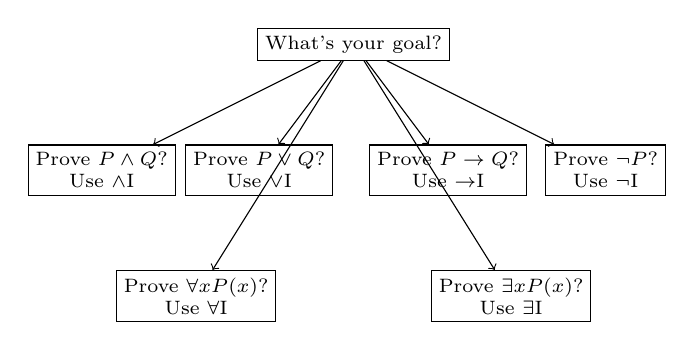
\begin{tikzpicture}[scale=0.8, every node/.style={rectangle, draw, align=center}]
			\scriptsize
			\node (root) at (0,0) {What's your goal?};
			\node (and) at (-4,-2) {Prove $P \land Q$?\\ Use $\land$I};
			\node (or) at (-1.5,-2) {Prove $P \lor Q$?\\ Use $\lor$I};
			\node (if) at (1.5,-2) {Prove $P \rightarrow Q$?\\ Use $\rightarrow$I};
			\node (not) at (4,-2) {Prove $\neg P$?\\ Use $\neg$I};
			\node (all) at (-2.5,-4) {Prove $\forall x P(x)$?\\ Use $\forall$I};
			\node (some) at (2.5,-4) {Prove $\exists x P(x)$?\\ Use $\exists$I};
			
			\draw[->] (root) -- (and);
			\draw[->] (root) -- (or);
			\draw[->] (root) -- (if);
			\draw[->] (root) -- (not);
			\draw[->] (root) -- (all);
			\draw[->] (root) -- (some);
		\end{tikzpicture}
	\end{frame}
	
	% Slide 36: Common Proof Patterns
	\begin{frame}{Common Proof Patterns: Recognizing Standard Arguments}
		\begin{itemize}
			\item \textbf{Chain of implications}: Use repeated modus ponens to follow $P \rightarrow Q \rightarrow R$.
			\item \textbf{Proof by cases}: When given $P \lor Q$, show your goal follows from each option.
			\item \textbf{Universal to specific}: Apply general rules to particular individuals with $\forall$E.
			\item \textbf{Existence proof}: Find one example and use $\exists$I.
		\end{itemize}
		
		\begin{example}
			Classic patterns in Wonderland:
			\begin{itemize}
				\item "All cards are flat; the King is a card; so the King is flat" ($\forall$E + MP)
				\item "Either eat the cake or drink the potion; both lead to size change" ($\lor$E)
				\item "If late, then in trouble; late; therefore in trouble" (MP)
				\item "The Cheshire Cat can disappear; so something can disappear" ($\exists$I)
			\end{itemize}
		\end{example}
	\end{frame}
	
	% Slide 37: Tips for Getting Unstuck
	\begin{frame}{Tips for Getting Unstuck: What to Do When You're Lost}
		\begin{itemize}
			\item \textbf{List what you have}: Write down all premises and what you've proven so far.
			\item \textbf{Clarify your goal}: What exactly are you trying to prove? What's its structure?
			\item \textbf{Work backwards}: What would directly give you the conclusion? What would give you that?
			\item \textbf{Look for unused premises}: Every premise should typically be used in the proof.
		\end{itemize}
		
		\begin{alertblock}{Common Unsticking Techniques}
			\begin{itemize}
				\item Can't prove $P \rightarrow Q$? Try assuming $P$ and proving $Q$
				\item Can't prove $\neg P$? Try assuming $P$ and finding a contradiction
				\item Have $P \lor Q$ but stuck? Try both cases separately
				\item Can't prove $\forall x P(x)$? Prove it for an arbitrary individual
				\item Remember: Complex statements can often be broken into simpler parts!
			\end{itemize}
		\end{alertblock}
	\end{frame}
	
	% Slide 38: Checking Your Work
	\begin{frame}{Checking Your Work: How to Know Your Proof Is Complete}
		\begin{itemize}
			\item \textbf{Every line is justified}: Each step cites a rule and the exact lines it uses.
			\item \textbf{Rules applied correctly}: Check that you're using each rule properly.
			\item \textbf{Fresh names where required}: For $\forall$I and $\exists$E, ensure names are truly new.
			\item \textbf{Conclusion matches goal}: Your last line should be exactly what you set out to prove.
		\end{itemize}
		
		\begin{block}{Proof Checklist}
			\begin{enumerate}
				\item $\checkmark$ Are all premises listed and numbered?
				\item $\checkmark$ Does each line follow from previous ones?
				\item $\checkmark$ Are all subproofs properly closed?
				\item $\checkmark$ Are variable restrictions respected?
				\item $\checkmark$ Is the conclusion exactly what was required?
			\end{enumerate}
			If you can check all boxes, your proof is complete!
		\end{block}
	\end{frame}
	
	% Slide 40: Next Steps
	\begin{frame}{Next Steps: From Basic Proofs to Mathematical Reasoning}
		\begin{itemize}
			\item You've learned the fundamental rules of deductive reasoning—the foundation of all mathematical proof!
			\item These same techniques appear in: calculus proofs, computer science algorithms, philosophical arguments.
			\item Remember: Proof-writing is a skill that improves with practice—keep working problems!
		\end{itemize}
		
		\begin{block}{Where Proofs Will Take You}
			\begin{itemize}
				\item \textbf{Mathematics}: Prove theorems about numbers, shapes, and functions
				\item \textbf{Computer Science}: Verify algorithms work correctly every time
				\item \textbf{Philosophy}: Analyze arguments about knowledge, ethics, and reality
				\item \textbf{Science}: Distinguish between correlation and causation
			\end{itemize}
		\end{block}
		
	\end{frame}
\end{document}